\documentclass{beamer}

%\usepackage{beamerthemesplit}
\usepackage[brazil]{babel}
%\usepackage[utf8]{inputenc}
%\usepackage[T2A]{fontenc}
%descomente para ISO e comente as duas de cima
\usepackage[latin1]{inputenc}
%\usetheme{Frankfurt}
%\usetheme{Singapore}
\usetheme{Boadilla}
%\usetheme{Berkeley}
\useinnertheme{rounded}
\usefonttheme{structurebold}
\usepackage{latexsym}
\usepackage{verbatim}
\usepackage{graphicx}
\usepackage{epsfig}

%transparenz
\setbeamercovered{
still covered={\opaqueness<1>{15}\opaqueness<2>{10}
\opaqueness<3>{5}\opaqueness<4->{2}},
again covered={\opaqueness<1->{15}}
}
\setbeamertemplate{navigation symbols}{}


\title[Trabalho de Gradua��o]{ Experimentos de Pesquisa Multidimensional em �rvores \textit{K-D} e \textit{K-D-B} versus Banco de Dados Relacional }
\author[UFPR]{Luiz Francisco Artigas de Pr�\\ Renato Yamazaki \\ Saulo Quinteiro dos Santos}
\institute[DINF]{Universidade Federal do Paran� \\ \today}
\date[\today]{Orientador: Elias Proc�pio Duarte Jr. \\ Co-orientador: Andreas Kiefer}

\begin{document}

\frame{\titlepage}

%\section[Roteiro]{}
%\frame{\tableofcontents}

\AtBeginSection[]
{
    \begin{frame}
    	\frametitle{Roteiro}
	\tableofcontents[currentsection]
    \end{frame}
}

\section{Motiva��o}

\begin{frame}
	\frametitle{Porque comparar o MySQL com �rvores multidimensionais?}
	\begin{itemize}
		\item Aplica��es distribu�das possuem requisitos espec�ficos de desempenho, e para isso necessitam do gerenciamento da rede que oferece o servi�o.
		\item A ger�ncia de redes consiste no controle e monitora��o dos elementos de uma rede, para atingir uma melhor utiliza��o dos recursos e assegurar um certo n�vel de servi�o.
		\item A motiva��o � estudar a efici�ncia no armazenamento e pesquisa de informa��es gerenciais, em estruturas de dados diferentes.
	\end{itemize}
\end{frame}



\section{Pesquisa Multidimensional}

\begin{frame}
	\frametitle{}
	\begin{itemize}
		\item a
		\item b
		\item c
	\end{itemize}
\end{frame}

\section{�rvores Multidimensionais}

%%%%%%%%%%%%%%%%%%%%%%%%%%%%%%%%%%%%%%%%%%%%%%%%%%%%%%%%%%%%%%%%%%%%%%%%%%%%%%%%
\begin{frame}
	\frametitle{�rvore \textit{K-D}}
	\begin{itemize}
		\item Semelhante � �rvore bin�ria, por�m possibilita a pesquisa por m�ltiplos atributos.
		\item Na �rvore \textit{K-D} os registros s�o definidos por \textit{K} chaves.
		\item A chave que determina a sub-�rvore que ser� acessada, varia a cada n�vel.
		\item No n�vel $L$ a chave $L\ mod\ (K+1)$ � utilizada.
	\end{itemize}
\end{frame}

\begin{frame}
	\frametitle{�rvore \textit{K-D}}
	\begin{figure}[h]
	\center
	\subfigure{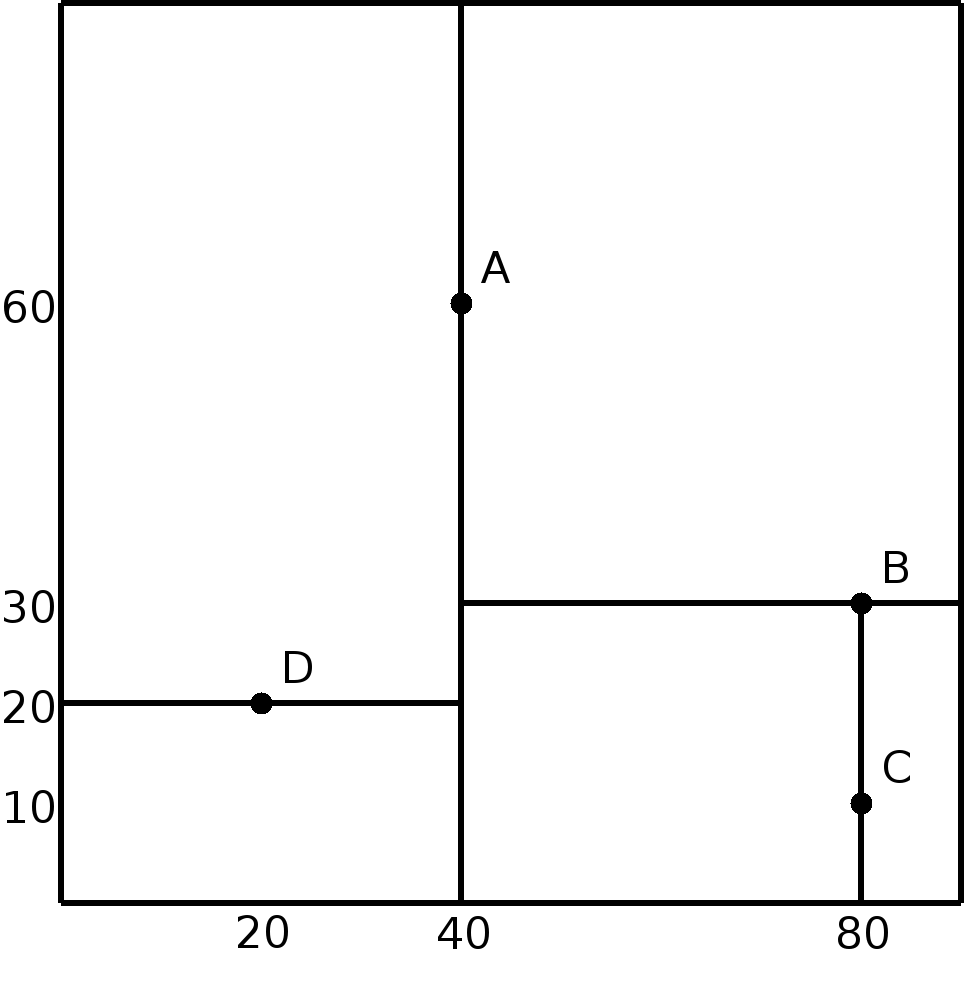
\includegraphics[width=5cm]{../images/algorithm/kd_plano.png}}
	\qquad
	\subfigure{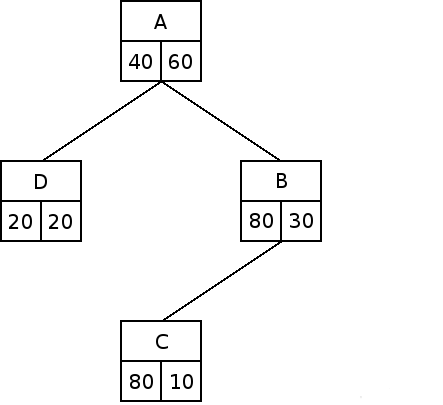
\includegraphics[width=5cm]{../images/algorithm/kd_passo4.png}}
	\end{figure}
\end{frame}

\begin{frame}
	\frametitle{�rvore \textit{K-D}: Opera��es}
	\textbf{Pesquisa}
	\begin{itemize}
		\item Pode ser classificada em pesquisa em exata, parcial ou por intervalo.
		\item Percorre a estrutura usando os crit�rios escolhidos (de acordo com o tipo de pesquisa).		
	\end{itemize}
	\textbf{Inser��o}
	\begin{itemize}
		\item Percorre a estrutura usando da pesquisa exata.
		\item Ao encontrar um n� folha, cria um n� com os novos dados e se torna filho do n� folha encontrado.
	\end{itemize}
\end{frame}

\begin{frame}
	\frametitle{�rvore \textit{K-D}: Inser��o}
	\begin{figure}[h]
	\center
	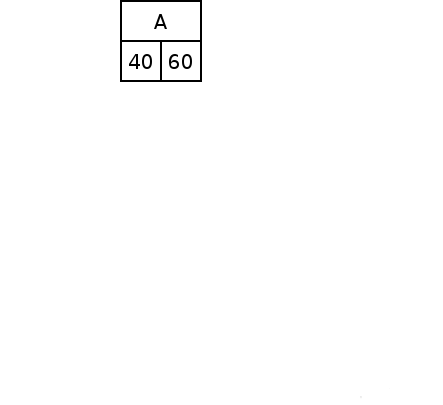
\includegraphics[width=7cm]{../images/algorithm/kd_passo1.png}
	\end{figure}
\end{frame}

\begin{frame}
	\frametitle{�rvore \textit{K-D}: Inser��o}
	\begin{figure}[h]
	\center
	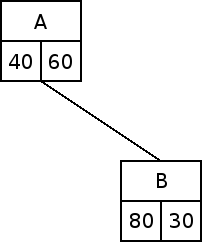
\includegraphics[width=7cm]{../images/algorithm/kd_passo2.png}
	\end{figure}
\end{frame}

\begin{frame}
	\frametitle{�rvore \textit{K-D}: Inser��o}
	\begin{figure}[h]
	\center
	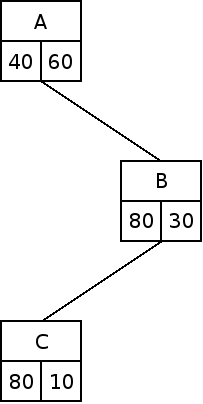
\includegraphics[width=7cm]{../images/algorithm/kd_passo3.png}
	\end{figure}
\end{frame}

\begin{frame}
	\frametitle{�rvore \textit{K-D}: Inser��o}
	\begin{figure}[h]
	\center
	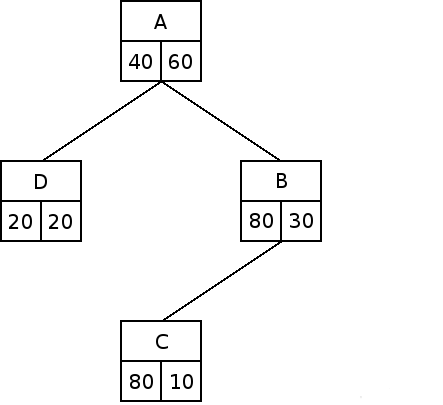
\includegraphics[width=7cm]{../images/algorithm/kd_passo4.png}
	\end{figure}
\end{frame}

\begin{frame}
	\frametitle{�rvore \textit{K-D}: Inser��o}
	\begin{figure}[h]
	\center
	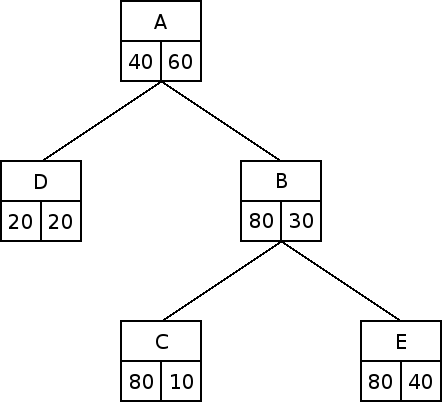
\includegraphics[width=7cm]{../images/algorithm/kd_passo5.png}
	\end{figure}
\end{frame}
%%%%%%%%%%%%%%%%%%%%%%%%%%%%%%%%%%%%%%%%%%%%%%%%%%%%%%%%%%%%%%%%%%%%%%%%%%%%%%%%
\begin{frame}
	\frametitle{�rvore \textit{K-D Adaptativa}}
	\begin{itemize}
		\item Varia��o da �rvore \textit{K-D}, resolve o problema do desbalanceamento utilizando o algoritmo de Hoare.
		\item O algoritmo encontra a mediana sobre os pontos da parti��o, para que a nova parti��o tenha o mesmo n�mero de pontos.
		\item Funciona melhor se os dados s�o conhecidos a priori.
	\end{itemize}
\end{frame}

\begin{frame}
	\frametitle{�rvore \textit{K-D Adaptativa}}
	\begin{figure}[h]
	\center
	\subfigure{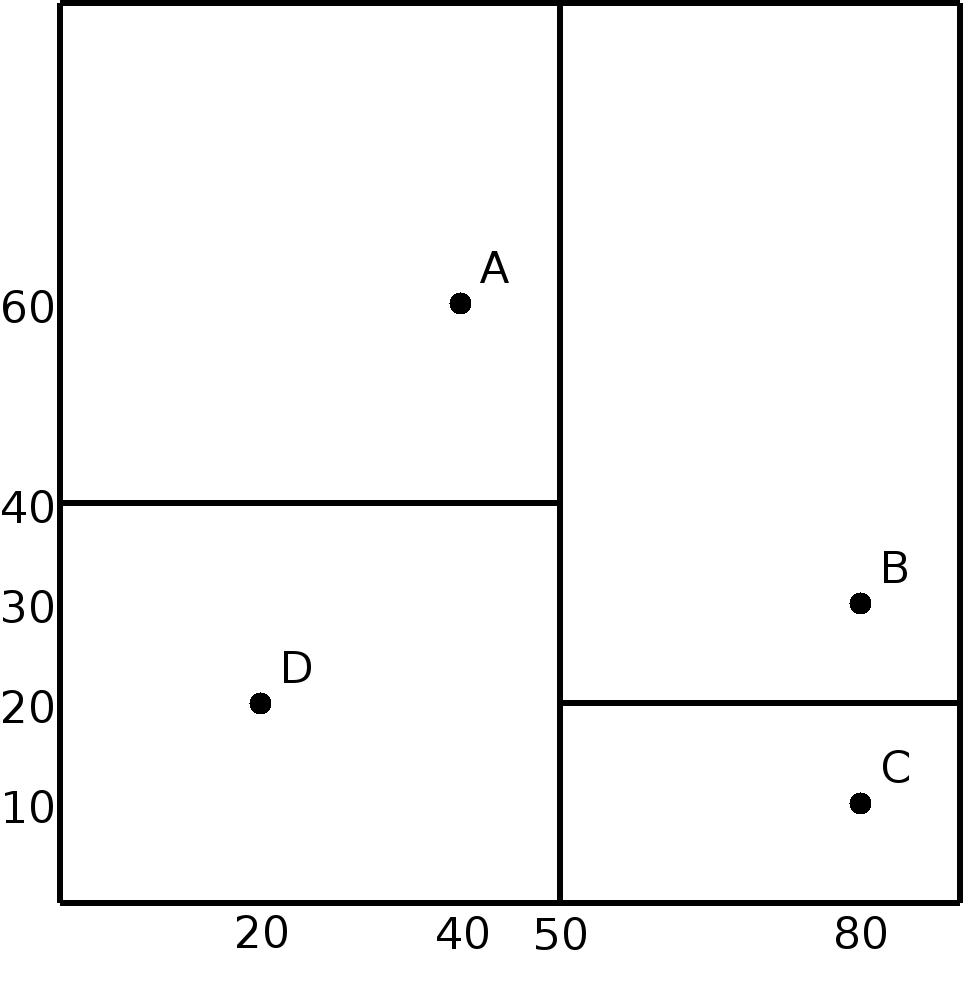
\includegraphics[width=5cm]{../images/algorithm/kda_plano.png}}
	\qquad
	\subfigure{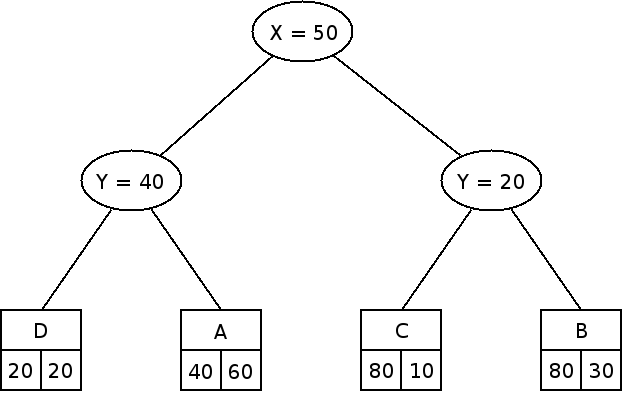
\includegraphics[width=5cm]{../images/algorithm/kda_1.png}}
	\end{figure}
\end{frame}

\begin{frame}
	\frametitle{�rvore \textit{K-D Adaptativa}: Opera��es}
	\textbf{Pesquisa}
	\begin{itemize}
		\item Semelhante ao algoritmo de pesquisa da �rvore \textit{K-D}. Possui os mesmos tipos de pesquisa: exata, parcial e por intervalo.
		\item Por�m, utiliza a mediana entre os pontos do plano atual, ao inv�s da chave do n� atual.
	\end{itemize}
	\textbf{Inser��o}
	\begin{itemize}
		\item Segue o mesmo racioc�nio da pesquisa, utilizando a pesquisa exata.
		\item Ao encontrar um n� folha, cria um n� com os novos dados e se torna filho do n� folha encontrado.
	\end{itemize}
\end{frame}

\begin{frame}
	\frametitle{�rvore \textit{K-D Adaptativa}: Inser��o}
	\begin{figure}[h]
	\center
	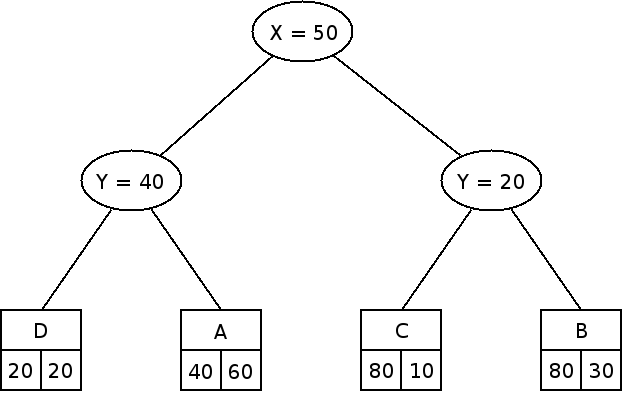
\includegraphics[width=10cm]{../images/algorithm/kda_1.png}
	\end{figure}
\end{frame}

\begin{frame}
	\frametitle{�rvore \textit{K-D Adaptativa}: Inser��o}
	\begin{figure}[h]
	\center
	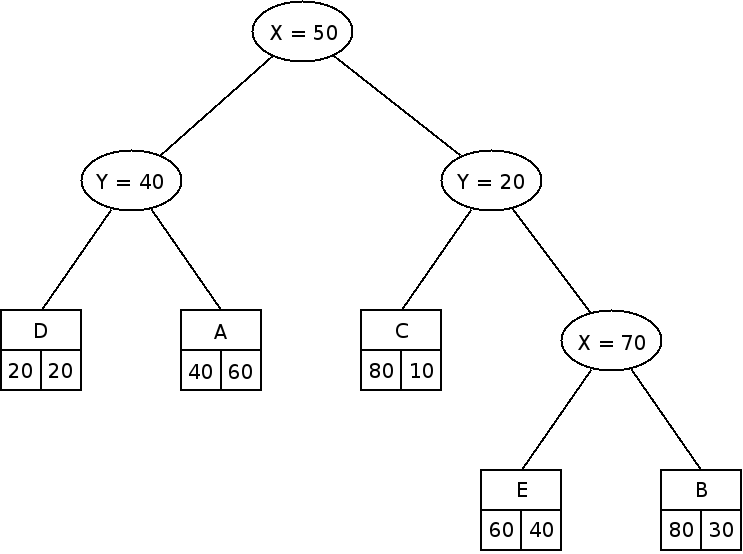
\includegraphics[width=10cm]{../images/algorithm/kda_2.png}
	\end{figure}
\end{frame}
%%%%%%%%%%%%%%%%%%%%%%%%%%%%%%%%%%%%%%%%%%%%%%%%%%%%%%%%%%%%%%%%%%%%%%%%%%%%%%%%
\begin{frame}
	\frametitle{�rvore \textit{K-D-B}}
	\begin{itemize}
		\item Possui caracter�sticas de �rvore \textit{K-D adaptativa} e �rvore \textit{B}.
		\item Os n�s internos s�o apontadores e representam determinada regi�o. S�o chamados de \textit{p�ginas de regi�es} e cont�m o endere�o para o n� filho.
		\item Os dados (pontos) s�o armazenados somente nas \textit{p�ginas de pontos} (folhas).
		\item As folhas est�o sempre em um mesmo n�vel, e isso garante que a �rvore esteja balanceada.
	\end{itemize}
\end{frame}

\begin{frame}
	\frametitle{�rvore \textit{K-D-B}}
	\begin{figure}[h]
	\center
	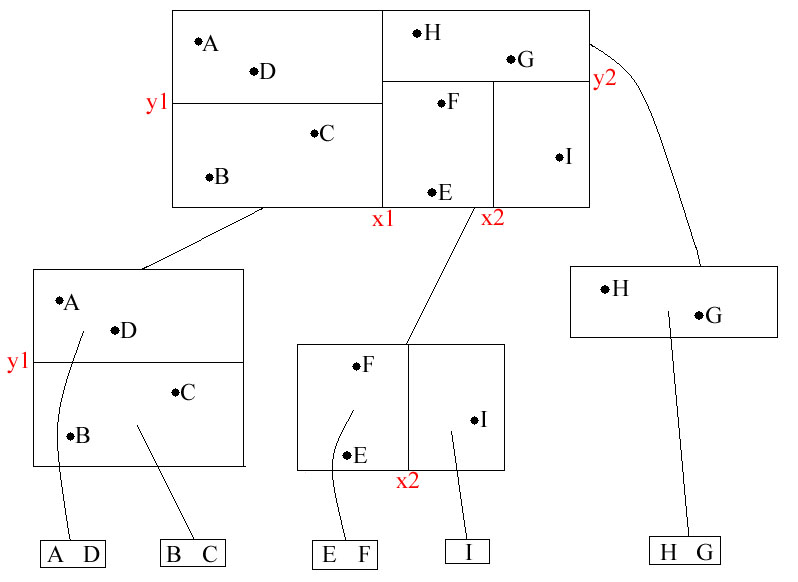
\includegraphics[width=10cm]{../images/kdb.jpg}
	\end{figure}
\end{frame}

\begin{frame}
	\frametitle{�rvore \textit{K-D-B}: Opera��es}
	\textbf{Pesquisa}
	\begin{itemize}
		\item Pode ser classificada em pesquisa exata, parcial e por intervalo.
		\item Os algoritmos de pesquisa fazem um caminho sobre a �rvore at� achar a p�gina de folha, usando a divis�o dos planos.
	\end{itemize}
	\textbf{Inser��o}
	\begin{itemize}
		\item Para inserir um ponto $p$ na �rvore, � localizada a p�gina folha apropriada para o ponto. Se existe espa�o na p�gina folha, $p$ � inserido, caso n�o, a p�gina � dividida em duas.
	\end{itemize}
\end{frame}

\section{Banco de Dados Relacional}

\begin{frame}
	\frametitle{Banco de dados Relacional}
	\begin{itemize}
		\item Bancos de dados, s�o conjuntos de registros dispostos em estrutura regular que possibilitam a reorganiza��o dos mesmos e produ��o de informa��o.
		\item Um banco de dados relacional � um conceito abstrato que define
	maneiras de armazenar, manipular e recuperar dados estruturados unicamente
	na forma de tabelas. 
		\item A tabela � um conjunto de dados dispostos em n�mero
	finito de colunas e n�mero ilimitado de linhas (ou tuplas).
	\end{itemize}
\end{frame}


\begin{frame}
	\frametitle{SGBD Sistema Gerenciador de Bando de Dados}
	\begin{itemize}
		\item � um conjunto de programas respons�vel pelo gerenciamento de uma base de dados que disponibiliza uma interface para incluir, alterar ou consultar dados.
		\item Essa interface � constitu�da pelas APIs ou drivers do SGBD, que executam comandos na linguagem SQL
	\end{itemize}
\end{frame}


\begin{frame}
	\frametitle{MySQL}
	\begin{itemize}
		\item O MySQL � um SGBD bastante popular, distribu�do como
	software livre, que utiliza a linguagem SQL como interface.
		\item Possui diversas estrat�gias de armazenamento dos dados, estas estrat�gias s�o chamadas de \textit{Storage Engine}, est�o entre elas \textit{MyISAM} e o \textit{InnoDB}.
		\item Ambas as \textit{Storage Engine} possibilitam a cria��o de �ndices com m�ltiplas chaves (at� 15 chaves).
	\end{itemize}
\end{frame}


\begin{frame}
	\frametitle{�ndices}	
	\begin{itemize}
		\item S�o estruturas de dados independentes que armazenam informa��es referentes �s chaves indexadas, de forma a referenciar o local onde est�o armazenados os dados.
		\item � comumente utilizada a �rvore B+ para armazenar os �ndices, pois ela apresenta a forma de uma �rvore balanceada e tem a poss�bilidade de acesso sequencial aos dados.
	\end{itemize}
	
\end{frame}


\begin{frame}
	\frametitle{�ndices: �rvore \textit{B+}}
	\begin{figure}[h]
	\center
	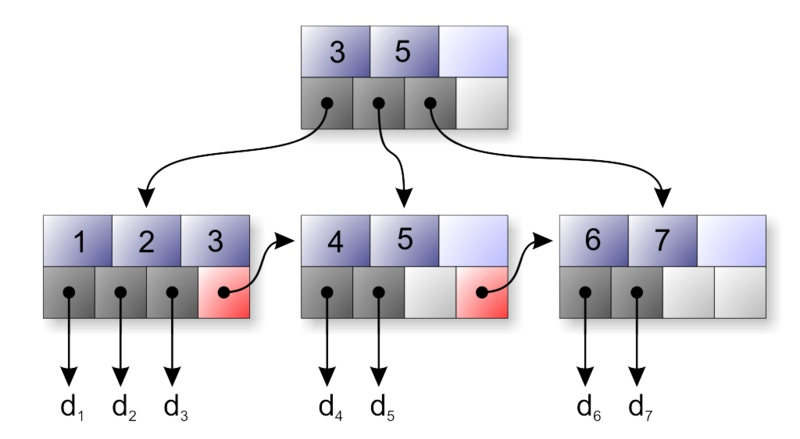
\includegraphics[width=10cm]{../images/arvorebmais.jpg}
	\end{figure}
\end{frame}


\begin{frame}
	\frametitle{MySQL: Opera��es}
	\textbf{Pesquisa}
	\begin{itemize}
		\item � poss�vel realizar diversos tipos de consulta no MySQL utilizando o comando SELECT da linguagem SQL.
		\item As consultas podem ser otimizadas, associando �ndices relacionados a chaves de busca � tabela.
	\end{itemize}
	\textbf{Inser��o}
	\begin{itemize}
		\item � feita atrav�s do comando INSERT da linguagem SQL.
		\item Para inserir dados carregados de um arquivo texto � poss�vel otimizar a inser��o de dados utilizando o LOAD DATA INFILE. 
	\end{itemize}
\end{frame}


\section{Experimentos}

\begin{frame}
	\frametitle{Decis�es de Implementa��o}
	\begin{itemize}
		\item Para a medi��o do tempo foi utilizada a fun��o \textit{clock()} da biblioteca \textit{time.h}.
		\item Experimento de compara��o entre arquivo de entrada bin�rio e texto.
		\item Nos arquivos de entrada texto, cada linha representa um dado multidimensional, e cada coluna uma dimens�o desse dado.
		\item N�mero de registros variam entre 16 mil, 100 mil, 250 mil, 500 mil, 1 milh�o, 2 milh�es, 4 milh�es e 8 milh�es. 
	\end{itemize}
\end{frame}

\begin{frame}
	\frametitle{Compara��o da �rvore K-D com o MySQL}
	\begin{itemize}
		\item Motiva��o: monitoramento \textit{online}.
		\item Biblioteca libkdtree++.
		\item Registro de 4, 8 e 16 chaves.
	\end{itemize}
\end{frame}

\begin{frame}
	\frametitle{Compara��o da �rvore K-D com o MySQL: Inser��o}
	\begin{figure}[h]
	\center
	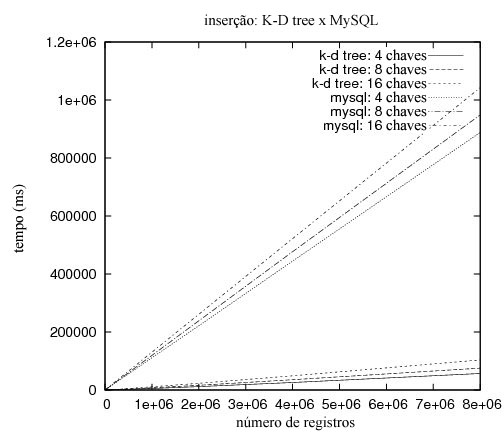
\includegraphics[width=10cm]{../images/experiments/Xkeys_insertion_kdtree_mysql.jpg}
	\end{figure}
\end{frame}

\begin{frame}
	\frametitle{Compara��o da �rvore K-D com o MySQL: Inser��o}
	\textbf{Resultados}\\
	\begin{itemize}
		\item Crescimento linear mais acentuado para o MySQL. 
		\item Pouca varia��o entre diferentes n�meros de chaves.
	\end{itemize}
\end{frame}

\begin{frame}
	\frametitle{Compara��o da �rvore K-D com o MySQL: Pesquisa}
	\begin{figure}[h]
	\center
	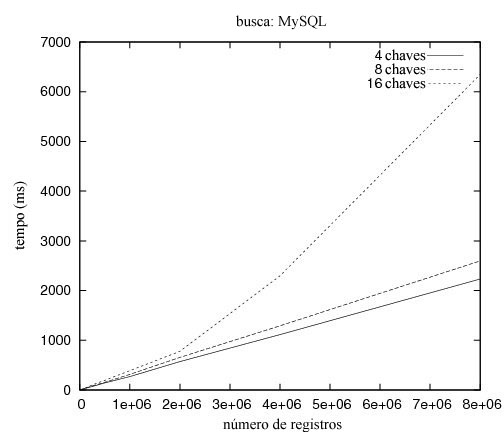
\includegraphics[width=10cm]{../images/experiments/Xkeys_search_mysql.jpg}
	\end{figure}
\end{frame}

\begin{frame}
	\frametitle{Compara��o da �rvore K-D com o MySQL: Pesquisa}
	\textbf{Resultados}\\
	\begin{itemize}
		\item Tempo de pesquisa da �rvore \textit{K-D}, menor que 2 milisegundos, n�o foi representado no gr�fico. 
		\item A partir de 2 milh�es de registros e 16 chaves, a curva do MySQL tem um crescimento acentuado. 
	\end{itemize}
\end{frame}

\begin{frame}
	\frametitle{Compara��o da �rvore K-D-B com o MySQL}
	\begin{itemize}
		\item Motiva��o: monitoramento \textit{offline}.
		\item Biblioteca TPIE.
		\item Registro de 10 chaves.
	\end{itemize}
\end{frame}

\begin{frame}
	\frametitle{Compara��o da �rvore K-D-B com o MySQL: Inser��o}
	\begin{figure}[h]
	\center
	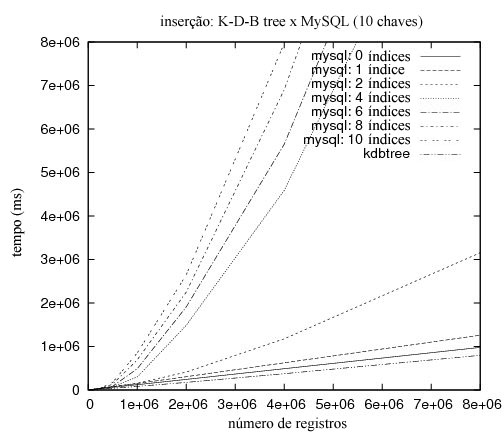
\includegraphics[width=8cm]{../images/experiments/10keys_insertion_kdbtree_mysql.jpg}
	\end{figure}
\end{frame}

\begin{frame}
	\frametitle{Compara��o da �rvore K-D-B com o MySQL: Inser��o}
	\textbf{Resultados}\\
	\begin{itemize}
		\item Para o MySQL, custo da opera��o acentuado proporcional ao n�mero de �ndices utilizados. 
		\item A �rvore \textit{K-D-B} mant�m o melhor desempenho.
	\end{itemize}
\end{frame}

\begin{frame}
	\frametitle{Compara��o da �rvore K-D-B com o MySQL: Inser��o}
	\begin{figure}[h]
	\center
	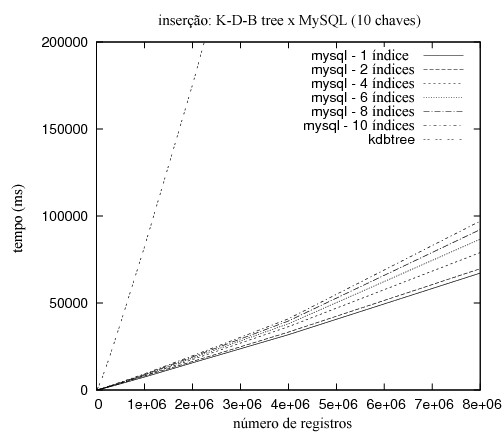
\includegraphics[width=8cm]{../images/experiments/10keys_insertion_kdbtree_mysql2.png}
	\end{figure}
\end{frame}

\begin{frame}
	\frametitle{Compara��o da �rvore K-D-B com o MySQL: Inser��o}
	\textbf{Resultados}\\
	\begin{itemize}
		\item O MySQL consegue tempos de inser��o muito baixos (1 minuto e 3 segundos para 8 milh�es de registros).
		\item A �rvore \textit{K-D-B} fez a inser��o de 8 milh�es de registros em 13 minutos e 24 segundos. 
	\end{itemize}
\end{frame}

\begin{frame}
	\frametitle{Compara��o da �rvore K-D-B com o MySQL: Pesquisa}
	\begin{figure}[h]
	\center
	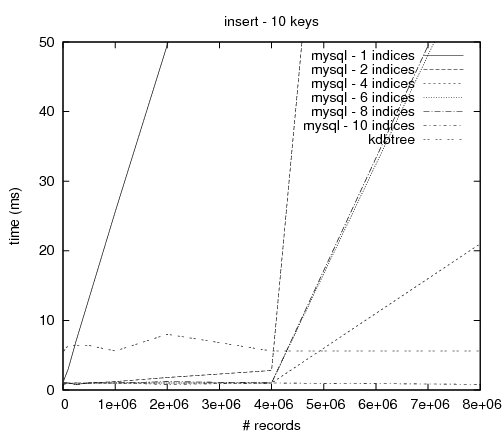
\includegraphics[width=8cm]{../images/experiments/10keys_search_kdbtree_mysql.jpg}
	\end{figure}
\end{frame}

\begin{frame}
	\frametitle{Compara��o da �rvore K-D-B com o MySQL: Pesquisa}
	\textbf{Resultados}\\
	\begin{itemize}
		\item Sem �ndices o MySQL leva 2,8 segundos para pesquisar em uma base de 8 milh�es de registros.
		\item Para a mesma base, a �rvore \textit{K-D-B} retorna o resultado em 5,6 milisegundos.
		\item O desempenho do MySQL melhora com o aumento do n�mero de chaves no �ndice.
		\item Com �ndice de 10 chaves, o MySQL se torna mais r�pido que a �rvore \textit{K-D-B}.
		\item Com menos chaves, o MySQL tem um crescimento acentuado a partir de 4 milh�es de registros. 
	\end{itemize}
\end{frame}


\section{Conclus�o}

\begin{frame}
	\frametitle{Conclus�o}
	\begin{itemize}
		\item a
		\item b
		\item c
	\end{itemize}
\end{frame}

\section{Trabalhos Futuros}

\begin{frame}
	\frametitle{Trabalhos Futuros}
	\begin{itemize}
		\item a
		\item b
		\item c
	\end{itemize}
\end{frame}


\end{document}
